\chapter{Conclusioni}

Il progetto sviluppato (in Figura \vref{fig:finalresult} è mostrato un esempio
della pagina finale) consente alle amministrazioni territoriali e ai cittadini
di \emph{controllare lo stato e l'andamento nel tempo della qualità dell'aria in
Italia}. Nella lotta all'inquinamento è fondamentale per le amministrazioni
avere uno strumento che consenta di \emph{valutare le strategie e gli
investimenti da adottare e, a posteriori, di controllare i risultati ottenuti}.

In Italia il tasso di motorizzazione è uno dei più alti nel mondo. Il passaggio
alla \standout{mobilità elettrica} sarà fondamentale per cercare di arginare il
problema dell'inquinamento dell'aria, ma non basta: le amministrazioni devono
anche provvedere a \standout{intervenire sull'industria}, affinché siano
adottate tecnologie innovative per ridurre le emissioni, e a
\standout{potenziare i servizi di trasporto pubblico} al fine di renderli più
attrattivi per i cittadini. In Italia, chi usa mezzi di trasporto pubblico
utilizza prevalentemente gli autobus, mentre ferrovie e metropolitane sono poco
impiegate, anche per il fatto che sono presenti solo in poche città italiane.

Uno strumento fondamentale è costituito dai \standout{Piani Urbani per la
Mobilità Sostenibile} (PUMS), uno strumento di \emph{pianificazione strategica}
che devono adottare tutte le amministrazioni territoriali con più di \(100000\)
abitanti.  I PUMS offrono l'opportunità di abbandonare la mobilità inquinante a
favore di una \emph{mobilità eco-sostenibile con mezzi a zero emissioni}, e di
\emph{cambiare progressivamente le abitudini dei cittadini} affinché impieghino
maggiormente, almeno per gli spostamenti intra-urbani, i mezzi di trasporto
pubblico.

Oggi il tema ambientale è molto sentito a livello sociale, come dimostrano i
movimenti nati recentemente, quale ad esempio \textsc{FridaysForFuture}, nel
tentativo di convincere i governi ad adottare efficaci misure per la tutela
dell'ambiente. Questa sensibilità verso la tutela ambientale permette di sperare
in una prossima rivoluzione \textit{eco-friendly}, affinché la protezione del
nostro pianeta e dell'ecosistema ricoprano un ruolo preminente e fondamentale.

\begin{figure}[p]
	\centering
	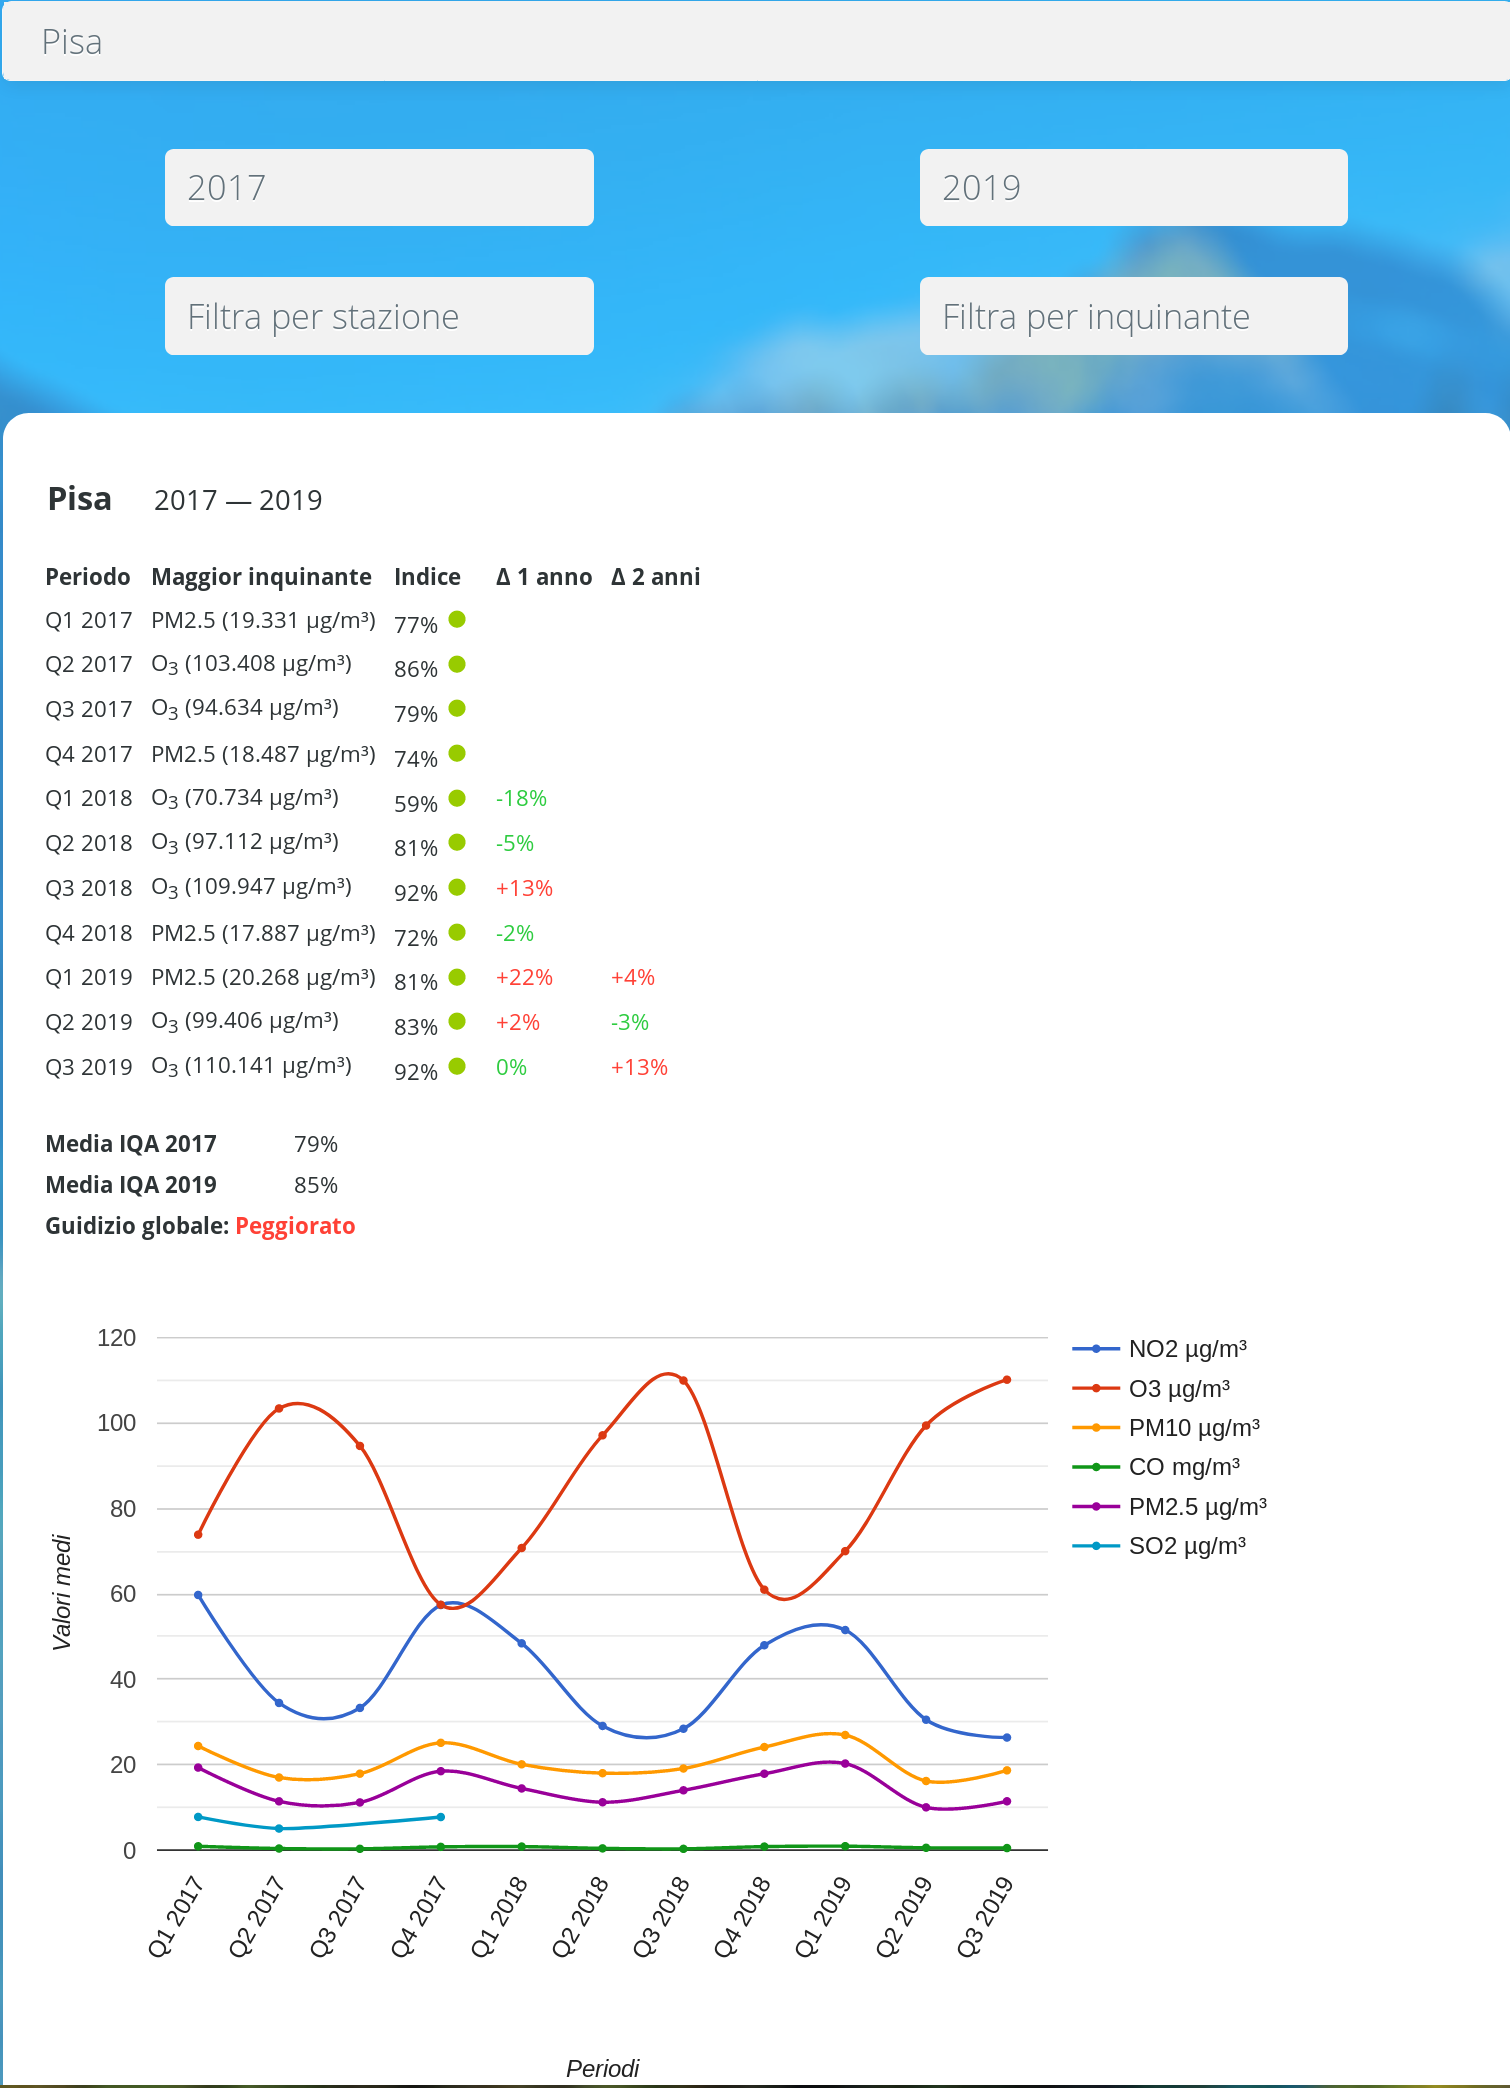
\includegraphics[width=\textwidth]{img/final-result}
	\caption{Pagina web finale del progetto realizzato. Esempio per la
	provincia di Pisa per il periodo 2017--2019.}\label{fig:finalresult}
\end{figure}
